\chapter{Présentation Générale}
\minitoc
\clearpage
%

\section{La Structure d'accueil}

\subsection{Présentation de HubSo}
HubSocial est une entreprise informatique créée en 2011. Le 01er Mai 2018, elle change de nom et devient HubSo. Elle œuvre pour le développement de solutions informatiques à valeurs sociales au Sénégal. Par l’usage des nouvelles technologies de l'information et de la communication, elle tente de matérialiser le concept d’actions sociales, d’aider les personnes et groupes les plus fragiles à mieux appréhender les domaines de la santé, de l’éducation, de la réduction de la pauvreté etc…\\
HubSo accompagne aussi d'autres entreprises à mettre en place des solutions informatiques qui leur sont adaptées. Sur ce point, HubSo étant un grand adepte du manifeste agile, tient à cœur la collaboration avec ces entités pour bâtir des partenariats solides plus que tout. De même, elle collabore aussi avec d'autres entreprises de services du numérique. Parmi ces collaborateurs de HubSo, nous avons : 
\begin{itemize}
	\itemtirait Intouch, le plus proche partenaire ;
	\itemtirait Mazars ;
	\itemtirait Yux ;
	\itemtirait Performances Group ;
	\itemtirait 2SI ;
	\itemtirait entre autres.
\end{itemize}

\subsection{Domaines d'activités}
HubSo propose les services suivants : 
\begin{itemize}
	\itemcheck Développement de solutions informatiques : HubSo est reconnue pour son expérience et ses références en matière de développement autour des technologies JEE et Android. Une équipe de plus de 15 ingénieurs de conception est à l'écoute de vos besoins; 
	\itemcheck Conseil en architecture d'entreprise : Les équipes de Hubso animent des ateliers avec ses clients  pour concevoir leur architecture d'entreprise; 
	\itemcheck Tierce maintenance applicative : aide à la maintenance d'application déjà en production et devant être corrigées ou améliorées; 
	\itemcheck Promotion de solutions innovantes pour la société : HubSo, c'est aussi l'innovation par la promotion de solutions.
\end{itemize}


\subsection{Quelques Solutions de HubSo }
HubSo propose entre autres, les solutions suivantes : 
\begin{itemize}
	\itemcheck TONGTONG \\
	TongTong est un site de vente en ligne basé sur les concepts d'achat groupé. TongTong, lancé par HubSo en 2014 , est aujourd'hui une référence dans le domaine de l'Ecommerce, notamment en matière de produits alimentaires manufacturés, de légumes, de produits locaux, etc. Il est possible de faire ses commandes sur www.tongtong.sn
	\itemcheck GRANT \\
	GRANT est une solution permettant à une entreprise de subventionner un ou plusieurs services pour ses employés. Elle a été lancée en 2017. Les subventions de tickets restaurant ont été intégrées à la plateforme et sont aujourd'hui utilisées par plusieurs entreprises.
	\itemcheck AVISJOURNAUX.COM \\
	AVISJOURNAUX.COM diffuse quotidiennement tous les appels d'offres et autres avis parus au Sénégal à ses milliers d'abonnés. C'est aujourd'hui une solution de référence dans le domaine, plébiscitée par les nombreux messages d'encouragement. Les abonnements "Grand public" sont gratuits. Cependant, une offre dédiée est commercialisée pour les regroupements de professionnels désirant bénéficier d'un service plus adapté. 
\end{itemize}

\subsection{Organisation}
\begin{figure}[h!]
	\centering
	\begin{minipage}{18cm}
		\centering
		{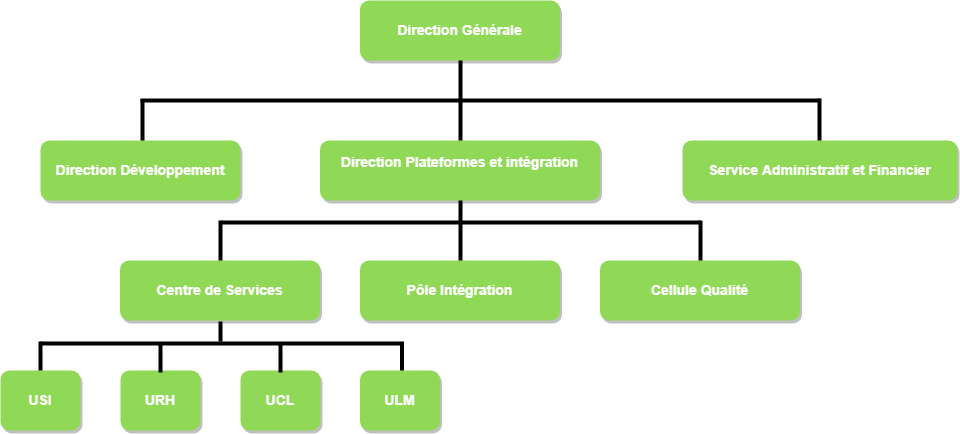
\includegraphics[height=0.27\textheight]{fig/Organnigramme-HubSo.png}}
	\end{minipage}
 	\caption{Organigramme de HubSo}
 	\label{fig:1.1}
\end{figure}
La figure \ref{fig:1.1} représente l'organigramme de HubSo. \\
HubSo comprend trois départements reliés à la Direction Générale : 
\begin{itemize}
	\itemcheck Direction Développement qui s'occupe du développement des solutions informatiques ; 
	\itemcheck Service Administratif et Financier s'occupant des affaires administratives et financières ;
	\itemcheck Direction plateformes et intégration qui comprend en son sein la Cellule Qualité chargée d'assurer la qualité des produits développés, le Pôle Intégration qui assure que tout produit développé répond aux exigences en matière de performance, de sécurité et de conformité par rapport aux différentes politiques de l'entreprise et le Centre de Services qui abrite l'Unité de Support Informatique (USI),l'Unité Logistique et Matérielle, l'Unité de Ressources Humaines et l'Unité de CL et dont le rôle est de mettre les employés dans les meilleures conditions et d'assurer un suivi des tâches de ces derniers grâce à un système de tickets.
\end{itemize}
Le Stage que nous avons réalisé s'est déroulé au niveau du Pôle Intégration.